%----------------------------------------------------------------------------------------
%	PACKAGES AND DOCUMENT CONFIGURATIONS
%----------------------------------------------------------------------------------------
\documentclass[11pt]{article}
\usepackage{amsmath} % Required for some math elements
\usepackage{hyperref} 
\usepackage{xcolor}
\usepackage{lipsum} 
\usepackage{cite}
\usepackage{graphicx} % Required for the inclusion of images
\usepackage{algorithmic}
\usepackage{array}
\usepackage{bookmark}
\usepackage{listings}
\usepackage{amssymb}
\usepackage{enumitem}
\usepackage[margin=24mm]{geometry}
\usepackage[caption=false, font=footnotesize]{subfig}
\usepackage{multirow}
\usepackage[active,tightpage]{preview}

\renewcommand{\PreviewBorder}{1in}
\newcommand{\Newpage}{\end{preview}\begin{preview}}

\newlist{steps}{enumerate}{1}
\setlist[steps, 1]{label = Step \arabic*:}

\hypersetup{ %color attributes of citation, link, etc.
    colorlinks=true,
    linkcolor=blue,
    filecolor=gray,      
    urlcolor=blue,
    citecolor=blue,
}


\definecolor{mGreen}{rgb}{0,0.7,0.5}
\definecolor{mWhite}{rgb}{0.9,0.9,0.9}
\definecolor{mGray}{rgb}{0.5,0.5,0.5}
\definecolor{mPurple}{rgb}{0.58,0,0.82}
\definecolor{backgroundColour}{rgb}{0.0,0.0,0.1}

\lstdefinestyle{Cstyle}{
    backgroundcolor=\color{backgroundColour},   
    commentstyle=\color{mGreen},
    keywordstyle=\color{magenta},
    numberstyle=\tiny\color{mGray},
    stringstyle=\color{mPurple},
    basicstyle=\footnotesize\color{mWhite},
    breakatwhitespace=false,         
    breaklines=true,                 
    captionpos=b,                    
    keepspaces=true,                 
    numbers=left,                    
    numbersep=5pt,                  
    showspaces=false,                
    showstringspaces=false,
    showtabs=false,                  
    tabsize=4,
    language=C
}


\newcommand{\matlab}{\textsc{Matlab }} %very important and totally necessary addition

\newcommand\Item[1][]{%
  \ifx\relax#1\relax  \item \else \item[#1] \fi
  \abovedisplayskip=0pt\abovedisplayshortskip=0pt~\vspace*{-\baselineskip}}
  %----------------------------------------------------------------------------------------
%	DOCUMENT INFORMATION
%----------------------------------------------------------------------------------------
 
\title{ECEN301 Embedded Systems Lab 3 \\ PWM, LDRs, Interrupts \& Timers Submission}
\author{Daniel Eisen 300447549}
\date{\today}

\begin{document}
\begin{preview}
\maketitle
%----------------------------------------------------------------------------------------
%	DOCUMENT CONTENT
%----------------------------------------------------------------------------------------
\section{Objectives}
The purpose of this lab was to introduce and familiarise the use of PWM generation, internal and external interrupts. The use of interrupts allows for events of interest to instantaiously be 'noticed' and trigger specific code in a section known as the 'Interrupt Service Routine.'

\section{Methodology}
        \subsection{Introduction}
        This lab consisted of 2 sections.
        One implemented simple PWM output with a varying duty cycle set by the IO box.
        The second utilised a comparator and light sensor to form a simple brightness level transducer
        \subsection{Part I: PWM Output}
        PWM generation on the 8051 utilises the PCA counters compare function. Therefore the PCA must be enabled (set CR bit), and the module in use (in this case 0) being set into PWM mode (PWN0, CCAPM0.1) with the compare function enabled (ECOM0, CCAPM0.6).

        \lstinputlisting[language=C,style=Cstyle]{../PWM_lab3/PWM_lab3/main.c}

        The duty cycle of the PWM output is set by loading an 8bit unsigned value input the CCAP0H registers, with 0 resulting in a 100\% cycle and 255 being near zero.

        \begin{center}
          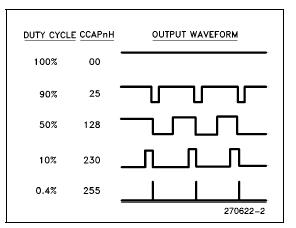
\includegraphics[width=0.39\textwidth]{inc/select duty cycle.jpg}
          \textit{\url{https://sites.google.com/site/controlandelectronics/pwm-tutorial-using-8051}}
        \end{center}

        To test the implementation, the IO module was connected to P0 to provide input to the duty cycle register and the output pin, CEX0, was probed with a scope.

        \begin{center}
          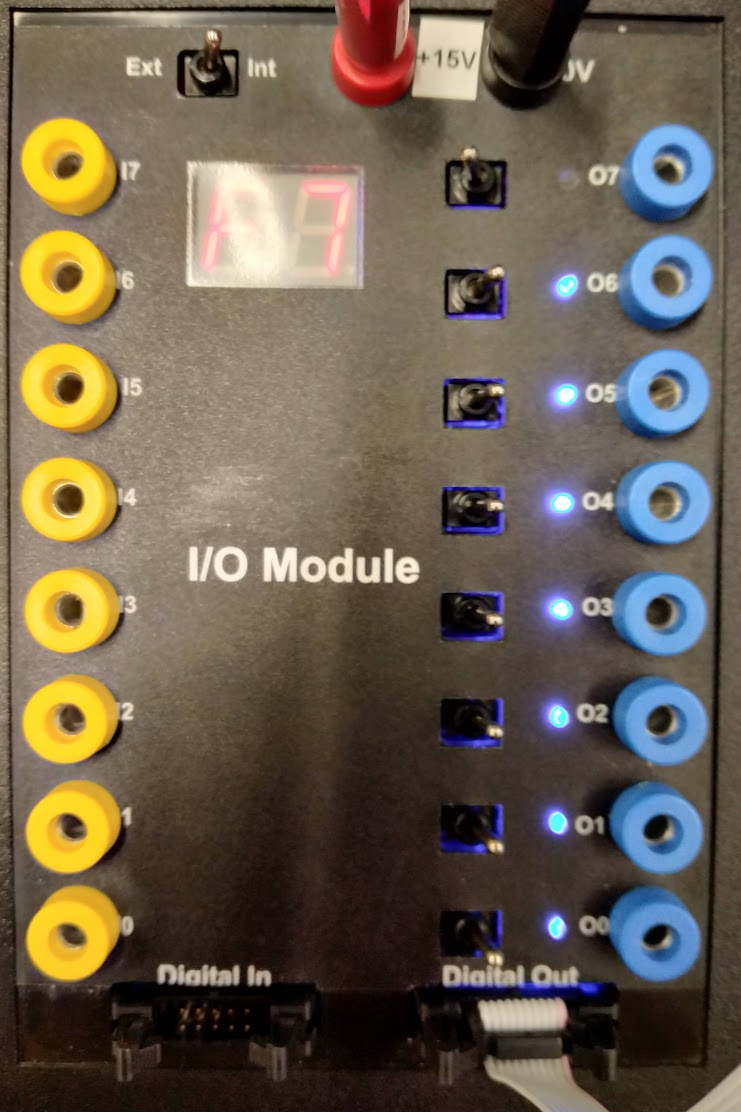
\includegraphics[width=0.2\textwidth]{inc/pwm_IP0.jpg}
          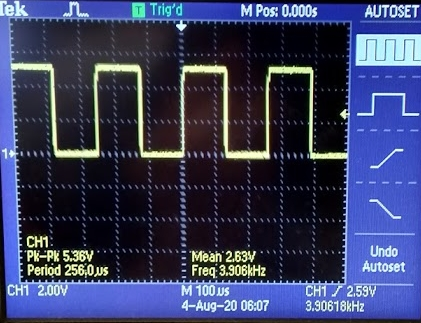
\includegraphics[width=0.39\textwidth]{inc/pwm_OP0.jpg}
        \end{center}

        Seen above is a 128 input the 50\% output.

        \begin{center}
          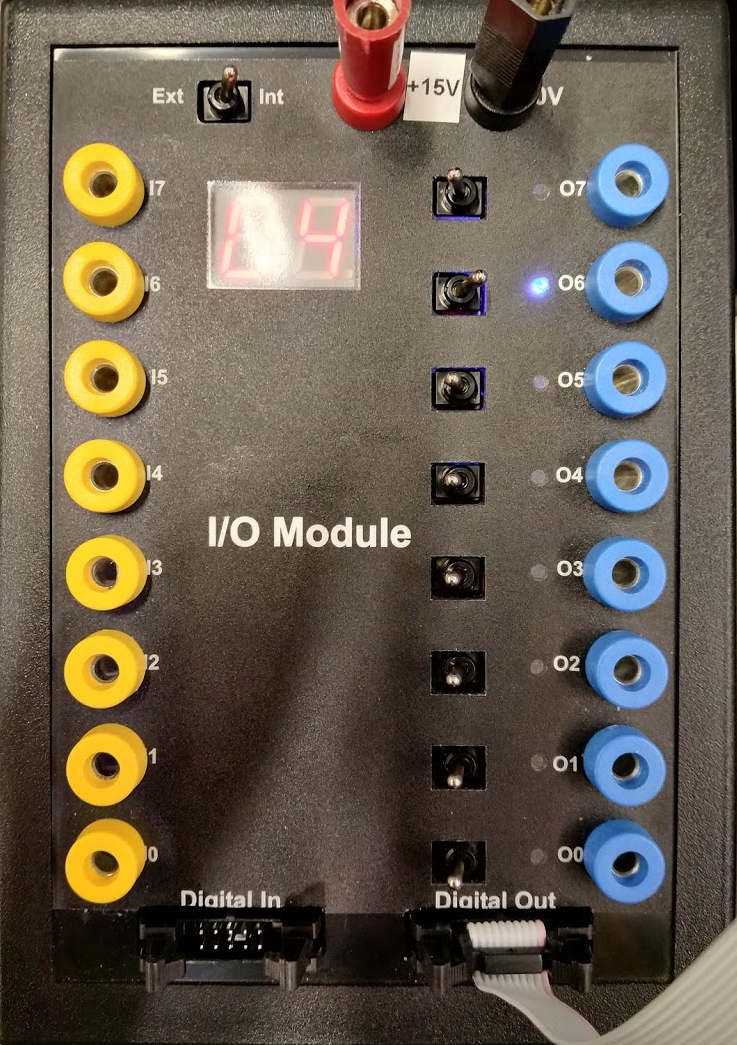
\includegraphics[width=0.2\textwidth]{inc/pwm_IP1.jpg}
          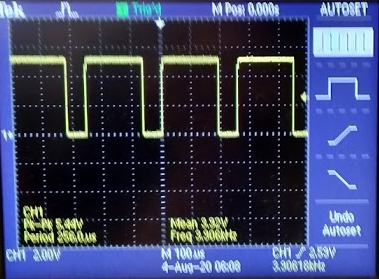
\includegraphics[width=0.39\textwidth]{inc/pwm_OP1.jpg}
        \end{center}
        
        Seen above is a 64 input the roughly 2 thirds duty cycle output.


        \subsection{Part II: LDRs and External Interrupts}
        To construct the brightness change transducer the main sensing unit used is a Light Dependent Resistor. Using this in a voltage divider, a light level dependant variable voltage can be extracted.

        To trigger an external interrupt, there must be either a falling or rising edge generated on the input pin to be detected. To translated the variable voltage into 2 distinct levels a comparator was used.

        Specifically the LM311 in its single supply operation. To put it simply there are 2 inputs, 1 is held constant and a varying signal is connected to the other. When the varying signal is large or smaller (in voltage) than the reference voltage the output will snap to either supply rail, in this case 5V or 0V. So when inputting the sensor voltage, then required edge can be generated when the light level sufficiently changes and an external interrupt can be triggered.

        \begin{center}
          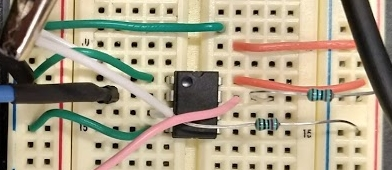
\includegraphics[width=0.6\textwidth]{inc/comp.jpg}
        \end{center}

        Above shows the comparator circuit as constructed. With measurement of the varying resistance of the LDR a 10K was chosen for the other side of the divider. Also due to the open-collector output of the LM311 the output is nominally pulled high through a 10K pullup.

        \lstinputlisting[language=C,style=Cstyle]{../INTRP_lab3/INTRP_lab3/main.c}

        Now that the hardware of the transducer is constructed and functional. The uC must be setup to enable external interrupts on the selected pin (with others disabled) and the relevant edge type set, in this case falling.
        
        A simple ISR just counts the number of interrupts generated, making the (wrong) assumption that accurately represents number of large light level changes and it then just displayed to the LCD panel as in previous labs.

        Notes: The interrupt flag is hardware cleared so the program doe not have to handle this.

        Due to output bouncing on the comparator output the count is in fact inaccurate, see Q.4 for more details.

\section{Questions}
\begin{enumerate}
        \item \textit{\textbf{What is meant by 'bit addressable'?}} \\
        This is an attribute of specific registers on the 8051. It describes the registers as being able to be set either with a full word, ie the full value of the entire register: \begin{verbatim}ADCON = 0b0000000\end{verbatim}
        Or each/some bits of the register can be set individually using its 'bit mnemonic':
        \begin{verbatim}PSIDLE=1 /*equivalent*/ ADCON |= 0b0100000\end{verbatim}
        
        \item \textit{\textbf{Explain what the bits of the CCAPMn and CMOD registers do.}}\\
        The CCAPMn are the special function registers that are associated with each of the modules in the PCA.
        \begin{enumerate}[label=Bit \arabic* ]\addtocounter{enumii}{-1}
          \item : ECCF, this enables or disables the CCON CCFx flag to allow for an interrupt request be generated when in match or compare mode.
          \item : PWM, this bit enables the pulse width modulation mode (on CEX output pin). 
          \item : TOG, when set the output pin CEX will toggle when a math
          \item : MAT, this sets when the PCA matches the capture/compare register. This triggers an interrupt when enabled.
          \item, 5 : CAPN,CAPP. These determine enable the edge type trigger of the capture mode. \textbf{P}ositive and/or \textbf{N}egative 
          \addtocounter{enumii}{1}
          \item : ECOM, enables comparator function.
          \item : Reserved
        \end{enumerate}
        The CMOD register is the PCA counter mode SFR.

        Bit 0 enables an interrupt to be generated when the PCA overflows, ie CCON:CF is set, others are reserved.

        Bits 2-1 are dedicated to selecting one of the sources for the PCA timer input; clk/6, clk/2, timer0 overflow, and external clk on P1.2.
        \item \textit{\textbf{What is the frequency, and how is it calculated?}}
        % (Hint: The PWM is using the bottom 8  bits  of  the  16  bit  PCA  counter,  and f_pca is  equal  to  half f_osc). How could you go about changing the frequency?
        The a internal clk frequency is 6Mhz, by default (CMOD = 0b00XXX000) the PCA input is 1/6, and with the PWM using the lower 8 of 16 bits:
        $$6Mhz/6/2^8 = 3.90625 kHz$$
        This is confirmed on the scope.
        \begin{center}
          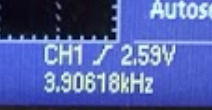
\includegraphics[width=0.5\textwidth]{inc/freq.png}
        \end{center}

        To change the frequency a different PCA input could be chosen, ie clk/2 or an external clock. But for greater control; using a auto-reloaded timer0 at varying values and using the overflow input can allow for varying the frequency in software.
        \item \textit{\textbf{Does switch bounce occur, and if so how do you deal with it?  Does your software restrict the number of interrupts you can generate in real time (i.e. is the software working at a restrictively slow pace)?}}\\
        Yes, bouncing occurred quite heavily, often counting upwards of 3 time per external trigger. The software itself does not handle, filter or attempt to mitigate the comparator bouncing in anyway and runs as fast as possible.

        To eliminate bouncing the LM311 can setup with hysteresis to allow for thresholding the output switching levels. This can be achieved with non-inverting feedback (R2) and input (R1) resistors to get:
        $$V_{TH} = ((R1+R2)*V_{ref}-(R1*V_{output-low}))/R2$$  
        $$V_{TL} = ((R1+R2)*V_{ref}-(R1*V_{output-high}))/R2$$  
        \label{bounce}
\end{enumerate}

\end{preview}
\end{document}